\documentclass[10pt]{article}
\usepackage[utf8]{inputenc}
\usepackage[T1]{fontenc}
\usepackage{graphicx}
\usepackage{tikz}
\usetikzlibrary{arrows}
\usepackage[export]{adjustbox}
\usepackage{amsmath}
\usepackage{amsfonts}
\usepackage{amssymb}
\usepackage[version=4]{mhchem}
\usepackage{stmaryrd}

\title{Data Structures and Algorithms Spring 2023 — Problem Sets }


\author{by Nikolai Kudasov}
\date{April 1, 2024}


\begin{document}
\maketitle

\section*{Week 11. Problem set}
\begin{enumerate}
  \item Write down all possible topological sortings for the nodes of the following directed graph:
\end{enumerate}

\begin{center}
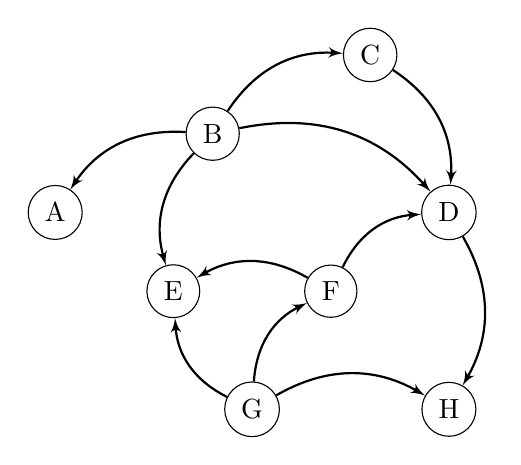
\begin{tikzpicture}

\tikzset{vertex/.style = {shape=circle,draw,minimum size=1.5em}}
\tikzset{edge/.style = {->,> = latex',thick}}
% vertices
\node[vertex] (a) at  (0,0)   {A};
\node[vertex] (b) at  (2,1)   {B};
\node[vertex] (c) at  (4,2)   {C};
\node[vertex] (d) at  (5,0)   {D};
\node[vertex] (e) at  (1.5,-1)  {E};
\node[vertex] (f) at  (3.5,-1)  {F};
\node[vertex] (g) at  (2.5,-2.5) {G};
\node[vertex] (h) at  (5,-2.5)  {H};
%edges
\draw[edge] (b) to[bend right] (a);
\draw[edge] (b) to[bend left] (c);
\draw[edge] (b) to[bend left] (d);
\draw[edge] (c) to[bend left] (d);
\draw[edge] (d) to[bend left] (h);
\draw[edge] (b) to[bend right] (e);
\draw[edge] (f) to[bend left] (d);
\draw[edge] (f) to[bend right] (e);
\draw[edge] (g) to[bend left] (e);
\draw[edge] (g) to[bend left] (f);
\draw[edge] (g) to[bend left] (h);
\end{tikzpicture}
\end{center}

\begin{enumerate}
  \setcounter{enumi}{1}
  \item Give an example of a directed graph $G=(V, E)$, a source vertex $s$, and a set of edges $T \subseteq E$ such that
\end{enumerate}

\begin{itemize}
  \item $T$ forms a tree and
  \item for each vertex $v \in V$, the unique simple path in the graph $(V, T)$ from $s$ to $v$ is a shortest path in $G$, yet
  \item the set of edges $T$ cannot be produced by running BFS on $G$, no matter how the vertices are ordered in the adjacency lists.
\end{itemize}

\end{document}